% =====================================================================================
%  Power System Case Studies with PyPSA
%  Load flow, operating limits and renewable integration in a Sahel context
%  Compile: pdflatex (twice)
% =====================================================================================
\documentclass[11pt,a4paper]{article}

\usepackage[utf8]{inputenc}
\usepackage[T1]{fontenc}
\usepackage{lmodern}
\usepackage{mathptmx}
\usepackage[english]{babel}
\usepackage[a4paper,margin=2.3cm,headheight=14pt]{geometry}
\usepackage{amsmath,amssymb}
\usepackage{graphicx}
\usepackage{booktabs,tabularx,array,multirow}
\usepackage{xcolor}
\usepackage{listings}
\usepackage{caption}
\usepackage{enumitem}
\usepackage{titlesec}
\usepackage{fancyhdr}
\usepackage{microtype}
\usepackage[most]{tcolorbox}
\usepackage[hidelinks]{hyperref}

\graphicspath{{../results/figures/}}
\definecolor{accent}{RGB}{42,120,214}
\definecolor{ink2}{RGB}{82,81,78}
\definecolor{codebg}{RGB}{246,246,243}

\setlist{nosep,leftmargin=1.4em}
\setlength{\parskip}{4pt}
\setlength{\parindent}{0pt}
\captionsetup{font=small,labelfont=bf}
\titleformat{\section}{\Large\bfseries}{\thesection}{0.8em}{}
\titleformat{\subsection}{\large\bfseries}{\thesubsection}{0.8em}{}
\titleformat{\subsubsection}{\normalsize\bfseries}{\thesubsubsection}{0.8em}{}

\pagestyle{fancy}
\fancyhf{}
\fancyhead[L]{\footnotesize PyPSA case studies}
\fancyhead[R]{\footnotesize\nouppercase{\leftmark}}
\fancyfoot[C]{\small\thepage}
\renewcommand{\headrulewidth}{0.4pt}

\lstset{basicstyle=\ttfamily\footnotesize, backgroundcolor=\color{codebg}, frame=single,
  rulecolor=\color{codebg}, columns=fullflexible, keepspaces=true, breaklines=true,
  commentstyle=\color{ink2}\itshape, keywordstyle=\color{accent}\bfseries,
  language=Python, xleftmargin=4pt, xrightmargin=4pt, aboveskip=6pt, belowskip=6pt}

\newtcolorbox{keybox}[1]{colback=white,colframe=accent,boxrule=0.6pt,arc=1pt,
  left=6pt,right=6pt,top=4pt,bottom=4pt,title={\small\bfseries #1},coltitle=white,colbacktitle=accent}
\newtcolorbox{sayit}{colback=codebg,colframe=codebg,arc=1pt,left=6pt,right=6pt,top=3pt,bottom=3pt}

\newcommand{\fig}[3]{\begin{figure}[htbp]\centering\includegraphics[width=#2\textwidth]{#1}\caption{#3}\end{figure}}

\begin{document}

% ------------------------------------------------------------------------------ title
\begin{titlepage}
\centering
\vspace*{2.2cm}
{\LARGE\bfseries Power System Case Studies with PyPSA\par}
\vspace{0.4cm}
{\Large Load flow, operating limits and renewable integration\\ in a Sahel context\par}
\vspace{1.4cm}
\begin{tabular}{l}
\toprule
Nine case studies, one problem type each: solving the load flow, power balance,\\
undervoltage, congestion and N-1 security, demand growth and voltage stability,\\
reverse power flow and hosting capacity, and two real-data planning cases\\
(Niamey grid with solar and storage, Agadez off-grid mini-grid).\\
\bottomrule
\end{tabular}
\vspace{1.6cm}

{\large KOUAME Koffi Fidèle\par}
\vspace{0.2cm}
{\normalsize IMP-EGH Master, Track 6 System Analysis\par}
\vspace{0.2cm}
{\normalsize \today\par}
\vfill
{\small\color{ink2}
Code, datasets and executed notebooks: folder \texttt{pypsa-case-studies/}.\\
All numbers in this report are produced by that code (PyPSA 1.4, HiGHS, pvlib).\\
Grid parameters of the Niamey and Agadez cases are fictitious and educational;\\
weather data are real (NASA POWER, 2023).\par}
\end{titlepage}

\tableofcontents
\clearpage

% ------------------------------------------------------------------------------ summary
\section*{Executive summary}
\addcontentsline{toc}{section}{Executive summary}

This report solves and explains nine power-system case studies with PyPSA. Each one isolates
\emph{one type of problem} that an engineer meets when studying a grid, states the exercise,
builds a PyPSA dataset (buses, carriers, generators, loads, lines and their time series
\texttt{loads\_t}, \texttt{generators\_t}), solves it, and interprets the result as an expert
would present it to a jury or to decision-makers.

\begin{center}\small
\begin{tabularx}{\textwidth}{@{}l>{\raggedright}p{3.0cm}X@{}}
\toprule
Case & Problem type & Main result \\
\midrule
CS00 & Non-linear equations & Newton converges quadratically to a simple root (8 digits in 5 steps) but only linearly to a double root (ratio 0.5); it fails where $f'=0$. \\
CS01 & Solving the AC load flow & 3-bus Newton-Raphson from scratch: $|U_3| = 0.951$ p.u., 4 iterations; identical to PyPSA ($10^{-15}$). Literal exercise data are infeasible. \\
CS02 & Power balance & 30 MW of PV cut the thermal output from 50.3 to 20.2 MW and the losses by 31 \%, but the evening peak stays on the thermal plant. \\
CS03 & Undervoltage & Remote bus at 0.919 p.u., 24 h a day; a 15 MVAr capacitor bank restores 0.959 p.u. and cuts the daily losses by 16 \%. \\
CS04 & Congestion, N-1 & Hot-season N-1 overload of 113 \%; security-constrained OPF fixes it for 54 \$/h; the AC re-check reveals a voltage collapse (0.75 p.u.) needing 62 MVAr. \\
CS05 & Demand growth, stability & Voltages look fine up to +30 \% but all reactive reserve is gone; maximum loadability +77 \% (vs a false +145 \% if limits are ignored). \\
CS06 & Reverse flow, hosting & Hosting capacity at the weak bus: 3 MW $\rightarrow$ 66 MW (lower set points) $\rightarrow$ 129 MW (PF 0.95); battery + reactive control remove all overvoltage. \\
CS07 & Real case A, planning & Niamey, hourly 2023: without imports, 333 MW PV + 196 MW/783 MWh battery cut cost by 22 \% and fuel by 68 \%. \\
CS08 & Real case B, energy access & Agadez mini-grid: PV + battery supply 94 \% of demand; cost 0.30 $\rightarrow$ 0.16 \$/kWh, robust to fuel prices. \\
\bottomrule
\end{tabularx}
\end{center}

\begin{keybox}{Five messages for decision-makers}
\begin{enumerate}
\item Having enough megawatts does not mean the power reaches the customers: voltage and
      reactive power usually bind before line capacity (CS03, CS05, CS06).
\item The first warning of a stressed grid is the loss of reactive reserve, not a low voltage (CS05).
\item Cheap fixes come first: capacitor banks, voltage set points, inverter reactive control
      and preventive redispatch solve most problems at a fraction of the cost of new lines (CS03, CS04, CS06).
\item Solar is the cheapest energy in every case studied; storage is what lets the system absorb it (CS07, CS08).
\item Linear (DC) optimisation must always be checked with the full AC load flow (CS04, CS07).
\end{enumerate}
\end{keybox}

\clearpage
% ------------------------------------------------------------------------------ 1
\section{Introduction}

\subsection{Purpose and approach}
The load flow is the basic tool of power-system analysis: for a given generation, demand and
network, it gives the steady-state voltages, flows and losses. The goal of this work is not
only to obtain numbers with PyPSA, but to understand each electrical problem, to explain the
results and to recommend actions, as an energy-systems engineer would. The case studies are
organised by \emph{problem type} rather than by network size (Table~\ref{tab:typology}).

\begin{table}[htbp]\centering\small
\caption{Problem types, networks and methods.}\label{tab:typology}
\begin{tabularx}{\textwidth}{@{}lXlX@{}}
\toprule
Case & Problem type & Network & Method \\
\midrule
CS00 & Solving $f(x)=0$ & scalar & Newton's method \\
CS01 & Solving the AC load flow & 3 buses (Exercise 5) & Newton-Raphson from scratch, PyPSA \texttt{pf} \\
CS02 & Power balance, slack, reactive power & 3 buses, Niamey context & AC load flow, 24 h real profile \\
CS03 & Undervoltage & 5 buses, Niamey context & AC load flow, remedy comparison \\
CS04 & Congestion, N-1 security, prices & IEEE 9-bus (MATPOWER) & DC-OPF, SC-OPF, AC N-1 \\
CS05 & Demand growth, voltage stability & IEEE 14-bus (MATPOWER, PGLib) & AC load flow, Q limits, PV curve \\
CS06 & Reverse flow, hosting capacity, storage & IEEE 14-bus + PV + battery & AC load flow, 24 h real profile \\
CS07 & Planning with variable renewables & 5 buses, 8760 h, real weather & Capacity-expansion LOPF, AC checks \\
CS08 & Off-grid sizing (energy access) & single bus, 8760 h, real weather & Capacity-expansion LOPF, sensitivity \\
\bottomrule
\end{tabularx}
\end{table}

\subsection{Environment and repository}
The work is reproducible with Python 3.11+ and the packages of \texttt{environment.yml}:
PyPSA 1.4, the HiGHS solver, pvlib, pandas, matplotlib, jupytext and nbconvert.

\begin{lstlisting}[language=bash]
conda env create -f environment.yml && conda activate pypsa-cases
python scripts/build_datasets.py      # rebuild the PyPSA CSV datasets
python scripts/run_all.py             # execute every case study -> notebooks/, results/
\end{lstlisting}

\begin{center}\small
\begin{tabularx}{\textwidth}{@{}lX@{}}
\toprule
Folder & Content \\
\midrule
\texttt{src/pscs/} & shared library: MATPOWER reader, Newton-Raphson, indicators, solar and demand models, chart style \\
\texttt{data/raw/} & official MATPOWER files, PGLib-OPF ratings, NASA POWER hourly weather, reference results \\
\texttt{data/networks/} & eight PyPSA datasets (CSV folders), each with a README \\
\texttt{scripts/} & one script per case study (source of the notebooks), dataset builder, runner \\
\texttt{notebooks/} & executed Jupyter notebooks with all outputs \\
\texttt{results/} & figures (PNG) and tables (CSV, JSON summaries) \\
\bottomrule
\end{tabularx}
\end{center}

\subsection{Data sources}
\begin{itemize}
\item \textbf{IEEE 9-bus and 14-bus systems}: official MATPOWER files \texttt{case9.m} and
      \texttt{case14.m}; thermal ratings of the 14-bus system from PGLib-OPF v23.07 (IEEE PES).
\item \textbf{Weather}: NASA POWER hourly data for 2023 (CERES SYN1deg irradiance, MERRA-2
      temperature and wind) for Niamey (13.51\,N, 2.11\,E) and Agadez (16.97\,N, 7.99\,E).
\item \textbf{Renewables.ninja}: the code reads Renewables.ninja PV files directly and uses
      them automatically when present (\texttt{data/raw/renewables\_ninja/}). The API could not be
      reached from the computing environment of this study, so the PV series were computed from
      NASA POWER with pvlib, using the same model chain as Renewables.ninja (section~\ref{sec:pv}).
      A script, \texttt{scripts/fetch\_renewables\_ninja.py}, downloads the ninja files with a
      free API token; re-running the notebooks then uses them.
\item \textbf{Teaching networks (CS02, CS03, CS07)}: fictitious parameters inspired by the
      Niamey context; they do not represent NIGELEC data.
\end{itemize}

% ------------------------------------------------------------------------------ 2
\section{Methods}

\subsection{AC load flow and Newton-Raphson}
For every bus $i$, with $Y_{ik} = G_{ik} + jB_{ik}$ the admittance matrix and
$\theta_{ik} = \theta_i - \theta_k$:
\begin{align}
P_i &= |V_i|\sum_k |V_k|\,(G_{ik}\cos\theta_{ik} + B_{ik}\sin\theta_{ik}),\\
Q_i &= |V_i|\sum_k |V_k|\,(G_{ik}\sin\theta_{ik} - B_{ik}\cos\theta_{ik}).
\end{align}
Bus types fix two of the four quantities: slack ($|V|$, $\theta$), PV ($P$, $|V|$), PQ ($P$, $Q$).
The unknowns are $\theta$ at PV and PQ buses and $|V|$ at PQ buses. Newton-Raphson solves
\begin{equation}
\begin{bmatrix} \partial P/\partial\theta & \partial P/\partial |V| \\ \partial Q/\partial\theta & \partial Q/\partial|V|\end{bmatrix}
\begin{bmatrix}\Delta\theta \\ \Delta|V|\end{bmatrix} =
\begin{bmatrix} P^{spec} - P(\theta,|V|) \\ Q^{spec} - Q(\theta,|V|)\end{bmatrix}
\end{equation}
from a flat start. Our own implementation (\texttt{src/pscs/newton.py}) is used to check
PyPSA. On the official MATPOWER cases the two agree to machine precision and reproduce the
published solutions (Table~\ref{tab:validation}).

\begin{table}[htbp]\centering\small
\caption{Validation of the PyPSA models.}\label{tab:validation}
\resizebox{\textwidth}{!}{\begin{tabular}{@{}lllr@{}}
\toprule
Case & Quantity & Reference & Deviation of PyPSA \\
\midrule
Exercise 5 (CS01) & all voltages, flows & own Newton-Raphson & $< 4\times10^{-15}$ \\
IEEE 9-bus & $P_{G1}$ = 71.64 MW, losses 4.641 MW & own NR, MATPOWER solution & $< 10^{-13}$ \\
IEEE 14-bus & slack 232.39 MW, losses 13.393 MW & own NR, pandapower & $< 10^{-13}$ \\
IEEE 14-bus & bus voltages & IEEE CDF stored solution & 0.0013 p.u. (rounding) \\
\bottomrule
\end{tabular}}
\end{table}

\subsection{The PyPSA data model and datasets}
\begin{sloppypar}A PyPSA network is a set of component tables. Static data sit in \texttt{n.buses},
\texttt{n.generators}, \texttt{n.loads}, \texttt{n.lines}, \texttt{n.transformers},
\texttt{n.storage\_units}, \texttt{n.carriers}; time series in \texttt{n.loads\_t.p\_set},
\texttt{n.generators\_t.p\_max\_pu}, \texttt{n.generators\_t.p\_set}, etc. Each dataset of
this study is a standard CSV folder that any PyPSA user can open:\end{sloppypar}

\begin{lstlisting}
import pypsa
n = pypsa.Network("data/networks/niamey_3bus")   # buses.csv, lines.csv, loads-p_set.csv ...
n.pf()                                            # one AC load flow per snapshot (24 h)
n.buses_t.v_mag_pu                                # voltages, p.u.
n.lines_t.p0                                      # active flow at the sending end, MW
\end{lstlisting}

\textbf{Unit conversion.} PyPSA stores line impedances in ohm and admittances in siemens.
With $Z_b = V_{nom}^2/S_b$: $r_\Omega = r_{pu} Z_b$, $x_\Omega = x_{pu} Z_b$,
$b_S = b_{pu}/Z_b$. Transformers keep per-unit values on their own rating $s_{nom}$. Unit
errors are the most frequent mistake in load-flow studies; the validation of
Table~\ref{tab:validation} protects against them.

\subsection{Reactive limits: PV to PQ switching}
PyPSA's load flow holds the voltage of PV buses whatever reactive power it takes. Real
generators cannot. We apply the standard iteration (\texttt{pscs.kpi.enforce\_q\_limits}):
after each load flow, a generator above $Q_{max}$ (below $Q_{min}$) becomes a PQ injection
fixed at its limit, and the load flow is repeated until no limit is violated.

\begin{lstlisting}
for g in pv_generators:
    if q[g] > q_max[g]:
        n.generators.loc[g, "control"] = "PQ"     # loses voltage control
        n.generators.loc[g, "q_set"] = q_max[g]   # stuck at its limit
\end{lstlisting}

\subsection{Optimisation: DC-OPF, security-constrained OPF, capacity expansion}
\texttt{n.optimize()} solves a linear (or quadratic) optimal power flow over all snapshots:
\begin{equation}
\min \sum_a c^{cap}_a \bar P_a + \sum_t\sum_g \left(c_{1,g}\,p_{g,t} + c_{2,g}\,p_{g,t}^2\right)
\end{equation}
subject to nodal balance, linearised flows $|P_{\ell,t}| \le s_{max,pu}\,s_{nom,\ell}$,
availability $p_{g,t} \le \bar P_g\,p_{max,pu,g,t}$ and storage dynamics. For capacity
expansion, $c^{cap}$ is the annuity of the investment plus fixed O\&M:
$c^{cap} = \text{CAPEX}\cdot\left(\frac{r}{1-(1+r)^{-L}} + \text{FOM}\right)$ with $r = 8\,\%$.
\texttt{n.optimize.optimize\_security\_constrained()} adds, for each outage $c$, the
post-contingency flows $P_\ell + \text{LODF}_{\ell c} P_c$. The dual of the nodal balance is
the locational marginal price.

\subsection{Solar model chain}\label{sec:pv}
PV output per kWp is computed with pvlib from NASA POWER hourly data: solar position at
mid-hour, Hay-Davies transposition to a south-facing plane tilted at the latitude, Faiman cell
temperature, PVWatts DC model ($-0.4\,\%/^\circ$C) and 10\,\% system losses (the
Renewables.ninja default). Results for 2023: Niamey 19.5\,\% capacity factor
(1\,710 kWh/kWp, lowest in August during the monsoon), Agadez 21.2\,\% (1\,857 kWh/kWp).

\subsection{Demand model}
No public hourly load series of the Niamey grid exists, so demand is \emph{modelled} with the
real temperature: $D(t) = k\,s(h)\,[1 + 0.025\max(T_{24}(t) - 25^\circ\text{C}, 0)]$, with a
daily shape $s(h)$ peaking at 19:00-20:00 (lighting, households, cooling) and $T_{24}$ the
24-hour mean temperature. The annual peak falls on 4 May 2023 at 19:00, in the hot season.
This is an explicit assumption, stated wherever demand matters.

% ------------------------------------------------------------------------------ CS00
\section{CS00 - Newton's method}
\textbf{Problem.} Solve $f(x) = 10x^2 - 2x^3 = 0$ by Newton's method (Exercise 5, Assignment 1).
$f'(x) = 20x - 6x^2$; roots $x = 0$ (double) and $x = 5$ (simple); $f'$ vanishes at $0$ and $10/3$.

\begin{table}[htbp]\centering\small
\caption{Five Newton iterations from $x_0 = 1$ and $x_0 = 4$.}
\begin{tabular}{@{}c rrrr c rrrr@{}}
\toprule
& \multicolumn{4}{c}{(a) $x_0 = 1$} && \multicolumn{4}{c}{(b) $x_0 = 4$}\\
\cmidrule{2-5}\cmidrule{7-10}
$k$ & $x_k$ & $f(x_k)$ & $f'(x_k)$ & $\Delta x$ && $x_k$ & $f(x_k)$ & $f'(x_k)$ & $\Delta x$ \\
\midrule
0 & 1.00000 & 8.00000 & 14.0000 & $-$0.57143 && 4.00000 & 32.0000 & $-$16.0000 & 2.00000 \\
1 & 0.42857 & 1.67930 & 7.46939 & $-$0.22482 && 6.00000 & $-$72.0000 & $-$96.0000 & $-$0.75000 \\
2 & 0.20375 & 0.39821 & 3.82586 & $-$0.10408 && 5.25000 & $-$13.7813 & $-$60.3750 & $-$0.22826 \\
3 & 0.09966 & 0.09735 & 1.93366 & $-$0.05034 && 5.02174 & $-$1.09643 & $-$50.8724 & $-$0.02155 \\
4 & 0.04932 & 0.02408 & 0.97179 & $-$0.02478 && 5.00019 & $-$0.00933 & $-$50.0075 & $-$0.00019 \\
5 & 0.02454 & & & && 5.00000 & & & \\
\bottomrule
\end{tabular}
\end{table}

\fig{cs00_newton_function.png}{0.72}{$f(x)$, the iterates and the first tangents of each run.}

\textbf{Interpretation.} From $x_0 = 1$ the method converges to the double root, but only
linearly: $x_{k+1} = x_k(10 - 4x_k)/(20 - 6x_k) \to x_k/2$, so the error halves at each step.
From $x_0 = 4$ it first overshoots to 6, then converges quadratically to 5 (8 exact digits
after 5 iterations). At $x_0 = 10/3$ the tangent is horizontal and the method fails; about half
of the starting points in $[-2, 8]$ end at each root. \emph{Link with load flows:} the Jacobian
replaces $f'$; a flat start is a good guess; several solutions may exist; a singular Jacobian
marks the voltage-collapse point (CS05).

% ------------------------------------------------------------------------------ CS01
\section{CS01 - Solving the AC load flow (Exercise 5)}
\textbf{Problem.} Three buses and three identical pi lines; bus 1 slack ($|U_1| = 1.00$),
bus 2 PV ($P_{G2} = 0.50$, $|U_2| = 1.05$), bus 3 PQ ($P_{D3} = 2.50$, $Q_{D3} = 1.00$ p.u.).

\textbf{Data check.} The exercise gives $\underline Y_{ik} = j0.1$ and $\underline Y^0_{ik} = -j8$.
Read literally, the series element would be a capacitor and the shunt an 8 p.u. reactor;
the Newton iteration diverges and, physically, a series admittance of 0.1 p.u. cannot carry
2.5 p.u. We use the swapped values (series $-j8$, total shunt $j0.1$, i.e. $j0.05$ per end);
reading both values as impedances gives the same qualitative answer ($|U_3| = 0.971$).

\textbf{Admittance matrix.} $Y_{ii} = 2(-j8) + 2(j0.05) = -j15.9$ and $Y_{ik} = +j8$.

\textbf{Load-flow problem.} Unknowns $\theta_2, \theta_3, |U_3|$; equations $P_2 = 0.5$,
$P_3 = -2.5$, $Q_3 = -1.0$ (no $Q_2$ equation: PV bus). Jacobian at the flat start:
\[ J_0 = \begin{bmatrix} 16.8 & -8.4 & 0 \\ -8.4 & 16.4 & 0 \\ 0 & 0 & 15.4 \end{bmatrix}. \]

\begin{table}[htbp]\centering\small
\caption{Newton-Raphson iterations (Exercise 5).}
\begin{tabular}{@{}crrrr@{}}
\toprule
Iteration & max $|$mismatch$|$ (p.u.) & $\theta_2$ ($^\circ$) & $\theta_3$ ($^\circ$) & $|U_3|$ (p.u.) \\
\midrule
0 & 2.5 & 0.0000 & 0.0000 & 1.00000 \\
1 & $2.08\times10^{-1}$ & $-$3.5782 & $-$10.5668 & 0.96753 \\
2 & $4.13\times10^{-3}$ & $-$3.6522 & $-$11.0830 & 0.95182 \\
3 & $1.85\times10^{-6}$ & $-$3.6530 & $-$11.0949 & 0.95149 \\
4 & $3.9\times10^{-13}$ & $-$3.6530 & $-$11.0949 & 0.95149 \\
\bottomrule
\end{tabular}
\end{table}

\textbf{Results.} $|U_3| = 0.951$ p.u., $\theta_2 = -3.65^\circ$, $\theta_3 = -11.09^\circ$;
$P_{G1} = 2.000$ p.u. (lossless lines: $P_{G1} = P_{D3} - P_{G2}$), $Q_{G1} = 0.047$ p.u.,
$Q_{G2} = 1.222$ p.u. Total losses $S_{v,ges} = 0 + j0.269$ p.u.: the series reactances
consume more reactive power than the line capacitances produce. PyPSA gives the same values
to $4\times10^{-15}$.

\fig{cs01_convergence.png}{0.62}{Quadratic convergence: the number of correct digits doubles at each iteration.}

% ------------------------------------------------------------------------------ CS02
\section{CS02 - Power sharing (3-bus, Niamey context)}
\textbf{Problem.} A thermal plant (slack, 1.02 p.u.), a city (50 MW + 20 MVAr at the peak) and a
30 MW PV plant, linked by 15-25 km 132 kV lines (100 MVA hot-season rating).

\begin{table}[htbp]\centering\small
\caption{Design point (city at its peak, PV at 30 MW).}
\begin{tabular}{@{}lrrrrrr@{}}
\toprule
Variant & $|V_2|$ & $|V_3|$ & thermal P (MW) & thermal Q (MVAr) & PV Q (MVAr) & losses (MW) \\
\midrule
No PV & 1.009 & 1.014 & 50.28 & 17.8 & 0.0 & 0.280 \\
PV, unity power factor & 1.011 & 1.017 & 20.19 & 17.5 & 0.0 & 0.192 \\
PV, voltage control (1.02) & 1.013 & 1.020 & 20.18 & 5.7 & 11.7 & 0.180 \\
\bottomrule
\end{tabular}
\end{table}

\textbf{Answers.} (1) Voltages are close to nominal and within 0.95-1.05 p.u. (2) PV cuts
the thermal output from 50.3 to 20.2 MW: the estimate $50 - 30 = 20$ MW is right to within the
losses. (3) At unity power factor the thermal plant supplies the reactive power; in
voltage-control mode the inverters give 11.7 MVAr, within the 13.7 MVAr capability of 33 MVA
inverters at full output. (4) Maximum loading 33\,\%. (5) Losses fall from 0.28 to 0.19 MW.

\fig{cs02_day_balance.png}{0.72}{Real day (4 May 2023, annual peak): the thermal plant follows demand minus solar.}

\textbf{Real day.} On the peak day the PV plant produces at most 20 MW (hot, hazy sky) and 15\,\%
of the daily energy. The peak occurs after sunset, so the thermal plant must still be sized for
50 MW and ramp steeply between 16:00 and 19:00. Solar saves fuel; without storage it does not
reduce the firm capacity needed.

% ------------------------------------------------------------------------------ CS03
\section{CS03 - Undervoltage at a remote industrial zone}
\textbf{Problem.} Five buses; the industrial zone (35 MW + 18 MVAr) is at the end of an 85 km
line. The exercise \emph{assumed} 0.92 p.u.; we compute it.

\fig{cs03_voltage_profile.png}{0.62}{Voltage profile: only bus 5 violates the limit; the worst case is the evening peak.}

$V_5 = 0.923$ p.u. with PV at 40 MW and $0.919$ p.u. at the evening peak without sun: the PV
plant, far from bus 5, hardly helps. On an 85 km line $X = 33\,\Omega$ and $R = 10\,\Omega$:
reactive power costs three times more voltage than active power ($\Delta V \approx (RP + XQ)/V$).

\begin{table}[htbp]\centering\small
\caption{Remedies at the evening peak.}
\begin{tabular}{@{}lrrl@{}}
\toprule
Remedy & $|V_5|$ (p.u.) & losses (MW) & assessment \\
\midrule
None & 0.919 & 3.18 & violates \\
Capacitor bank 15 MVAr at bus 5 & 0.959 & 2.72 & cheapest, fixes the cause \\
Plant set point 1.05 p.u. & 0.953 & 2.96 & uses up the upper margin \\
Second circuit on line 4-5 & 0.956 & 2.48 & best losses, most expensive \\
PV inverters Q-at-night (1.03 p.u.) & 0.942 & 3.22 & needs 68 MVAr $>$ 44 MVA: infeasible \\
SVC/STATCOM at bus 5 (0.97 p.u.) & 0.970 & 2.66 & 17.9 MVAr, precise, costlier \\
\bottomrule
\end{tabular}
\end{table}

The minimum bank is 11.8 MVAr (sensitivity 0.28\,\% of voltage per MVAr); a 15 MVAr bank in
three 5 MVAr steps is recommended. Over the real day, bus 5 is below 0.95 p.u. 24 hours out of
24 without action and never with the bank, with no overvoltage at night; daily losses fall
from 59.7 to 50.1 MWh.

\fig{cs03_remedies.png}{0.68}{Comparison of the remedies at the evening peak.}

% ------------------------------------------------------------------------------ CS04
\section{CS04 - Congestion and N-1 security (IEEE 9-bus)}
\textbf{Problem.} Hot-season ratings (15\,\% below MATPOWER values, an assumption) and an
evening peak 15\,\% above the base case. Generator costs are the quadratic MATPOWER costs.

\textbf{Economic dispatch.} G1 101.4 MW, G2 153.5 MW, G3 107.3 MW, 6\,429 \$/h, uniform nodal
price 27.30 \$/MWh. The intact grid is fine (maximum loading 73\,\%).

\textbf{N-1 screening (AC).} The loss of line 8-9 overloads line 5-6 to 113\,\% of its rating:
the dispatch is not N-1 secure. The loss of line 9-4 leaves bus 9 at 0.75 p.u.

\begin{figure}[htbp]\centering
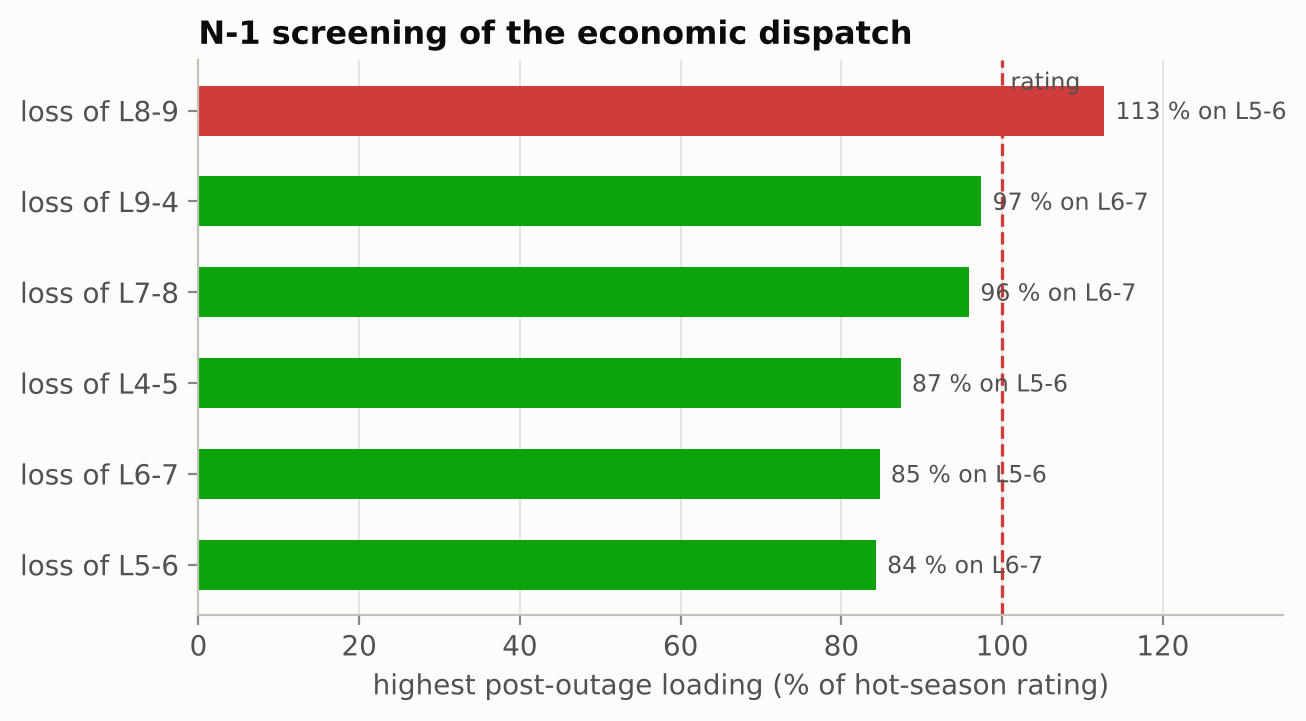
\includegraphics[width=0.49\textwidth]{cs04_n1_economic.png}\hfill
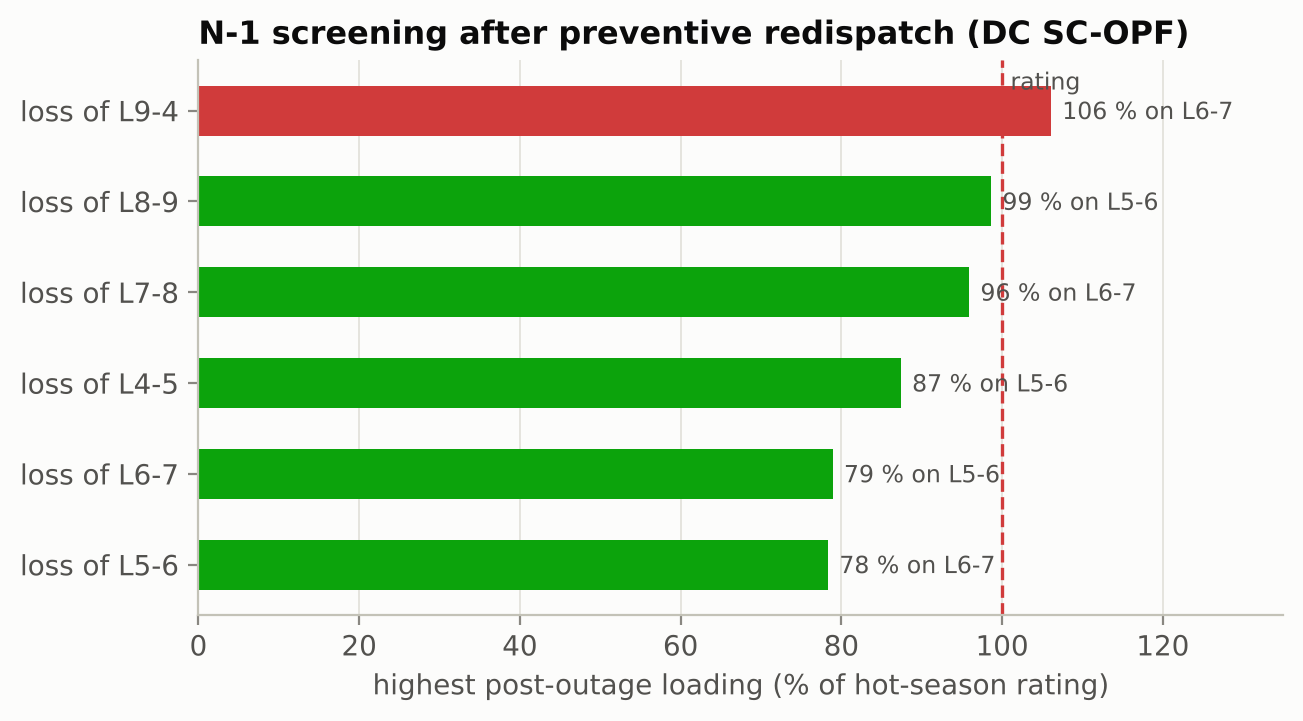
\includegraphics[width=0.49\textwidth]{cs04_n1_secure.png}
\caption{Worst post-outage loading for each line outage: economic dispatch (left) and after the security-constrained OPF (right).}
\end{figure}

\textbf{Preventive redispatch.} The security-constrained OPF moves 18 MW from G2 and G3 to G1:
G1 119.8, G2 142.7, G3 99.8 MW, for 54 \$/h (0.84\,\%). Nodal prices separate (25.5 to 31.3 \$/MWh):
the spread is the value of transport capacity. The AC re-check confirms 98.7\,\% on line 5-6,
but flags line 6-7 at 106\,\% after the loss of line 9-4: this is the voltage collapse at bus 9,
invisible to the DC model. 62 MVAr of reactive support switched in at bus 9 after that outage
restores 0.95 p.u. and brings line 6-7 back to 98.5\,\%.

\textbf{Redispatch or reinforce?} Uprating line 5-6 to 200 MVA makes the economic dispatch
N-1 secure for flows (worst 97\,\%) but does not cure bus 9. At 600 critical hours a year,
redispatch costs about 32 k\$/year: reinforcement is justified only if congestion becomes
frequent; the price spread tells the planner when.

% ------------------------------------------------------------------------------ CS05
\section{CS05 - Demand growth and voltage stability (IEEE 14-bus)}
\textbf{Problem.} All loads (and G2) grow by 10 to 50\,\%; generator reactive limits are enforced.

\begin{table}[htbp]\centering\small
\caption{Indicators per scenario (reactive limits enforced).}
\resizebox{\textwidth}{!}{\begin{tabular}{@{}lrrrrrr@{}}
\toprule
Scenario & min $|V|$ (p.u.) & buses $<$ 0.95 & max loading (\%) & losses (MW) & gen Q (MVAr) & units at Q limit \\
\midrule
S0 100\,\% & 1.010 & 0 & 59.1 & 13.4 & 82 & 0 of 4 \\
S1 110\,\% & 1.010 & 0 & 65.3 & 16.4 & 102 & 1 of 4 \\
S2 120\,\% & 1.006 & 0 & 71.7 & 19.8 & 123 & 3 of 4 \\
S3 130\,\% & 0.983 & 0 & 78.7 & 23.9 & 149 & 4 of 4 \\
S4 140\,\% & 0.954 & 0 & 86.6 & 28.9 & 179 & 4 of 4 \\
S5 150\,\% & 0.909 & 9 & 95.5 & 35.2 & 215 & 4 of 4 \\
\bottomrule
\end{tabular}}
\end{table}

\fig{cs05_pv_curve.png}{0.68}{PV (nose) curve at bus 14: maximum loadability +77\,\% with reactive limits.}

\textbf{Interpretation.} Up to +30\,\% the classic indicators look healthy, yet all four
voltage-controlling units reach their reactive limit: the reserve is exhausted. Beyond, voltages
fall fast (nine buses below 0.95 p.u. at +50\,\%) and losses grow with the square of the current
(13.4 to 35.2 MW). The maximum loadability is +77\,\% (458 MW); a 20 MVAr capacitor at bus 14
raises it to +81\,\%. Ignoring the reactive limits (PyPSA default) would wrongly suggest more than
+145\,\%. \emph{Recommendations:} reactive compensation at weak buses, voltage-control capability
on new plants, reinforcement of corridor 1-5, peak shaving.

% ------------------------------------------------------------------------------ CS06
\section{CS06 - Reverse power flow, hosting capacity and storage}
\textbf{Problem.} A PV plant at bus 14 of the IEEE 14-bus system (weakest node, local load
about 14 MW at noon), real solar profile of 16 March 2023; scenarios S0 to S4 of the exercise.

\begin{table}[htbp]\centering\small
\caption{Hosting capacity of bus 14 at the hour of maximum sun.}
\begin{tabular}{@{}lrl@{}}
\toprule
Strategy & Hosting capacity & First limit \\
\midrule
Unity PF, original IEEE voltage set points & 3 MW & overvoltage \\
Unity PF, generator set points $-0.03$ p.u. & 66 MW & overvoltage \\
PF 0.95 absorbing, set points $-0.03$ p.u. & 129 MW & undervoltage \\
\bottomrule
\end{tabular}
\end{table}

\fig{cs06_hosting_capacity.png}{0.95}{Voltage rise, not line capacity, limits solar at bus 14.}

\begin{table}[htbp]\centering\small
\caption{Twenty-four hour scenarios.}
\resizebox{\textwidth}{!}{\begin{tabular}{@{}lrrrrr@{}}
\toprule
Scenario & max $|V_{14}|$ & overvoltage hours & reverse-flow hours & max export (MW) & losses (MWh) \\
\midrule
S0 no PV & 1.057 & 15 & 0 & 0.0 & 211.0 \\
S1 PV 50 MW & 1.073 & 20 & 9 & 25.2 & 186.2 \\
S2 PV 100 MW & 1.098 & 20 & 10 & 62.4 & 180.2 \\
S3 S2 + battery 50 MW/200 MWh & 1.080 & 24 & 14 & 37.5 & 166.6 \\
S4 S3 + PF 0.95 + set points & 1.046 & 0 & 14 & 37.4 & 183.8 \\
\bottomrule
\end{tabular}}
\end{table}

\textbf{Interpretation.} The voltage plan comes first: with the original set points the customer
buses already exceed 1.06 p.u. at low load. Lowering the set points (free) and absorbing reactive
power multiply the hosting capacity by more than 40. The flow on lines 9-14 and 13-14 reverses as soon as PV
exceeds the local load. The battery (peak shaving) lowers the peak voltage and the export, but its
evening discharge at the weak bus raises the voltage there: storage needs a voltage-aware dispatch.
The full package (S4) removes every overvoltage hour.

\fig{cs06_day_v14.png}{0.66}{Voltage at bus 14 over the day for the five scenarios.}

% ------------------------------------------------------------------------------ CS07
\section{CS07 - Real case A: solar and storage for the Niamey area}
\textbf{Question.} How much PV and storage minimises the yearly cost of supply, with and without
imports, and what does it change for fuel, CO$_2$ and the grid? Hourly year 2023 (real weather,
modelled demand: 726 GWh, peak 105 MW), five-bus network of CS03 with the 15 MVAr bank. Costs:
PV 800 \$/kW (annualised 86.9 k\$/MW/yr), 4-hour battery 1\,150 \$/kW (157.4 k\$/MW/yr), thermal fuel
180 \$/MWh, imports 70 \$/MWh. When imports are interrupted the grid is an island and the thermal
plant keeps 20 MW online (must-run).

\begin{table}[htbp]\centering\small
\caption{Optimisation results (8760 hours of 2023).}
\resizebox{\textwidth}{!}{\begin{tabular}{@{}lrrrrrr@{}}
\toprule
Scenario & PV (MW) & battery (MW / MWh) & solar share & CO$_2$ (kt) & cost (M\$/yr) & \$/MWh \\
\midrule
A imports, no PV & 0 & 0 / 0 & 0\,\% & 35 & 56.4 & 77.6 \\
B no imports, no PV & 0 & 0 / 0 & 0\,\% & 508 & 130.7 & 180.0 \\
C no imports, 100 MW PV & 100 & 0 / 0 & 23\,\% & 391 & 109.3 & 150.5 \\
D0 no imports, optimal PV & 154 & 0 / 0 & 29\,\% & 361 & 106.2 & 146.2 \\
D no imports, optimal PV + battery & 333 & 196 / 783 & 72\,\% & 163 & 101.7 & 140.1 \\
E imports, optimal PV + battery & 144 & 8 / 33 & 33\,\% & 7 & 49.0 & 67.5 \\
\bottomrule
\end{tabular}}
\end{table}

\fig{cs07_cost_co2.png}{0.95}{Yearly cost and CO$_2$ emissions of the six scenarios.}
\fig{cs07_week_D.png}{0.95}{Scenario D in the hot season: solar by day, battery in the evening, thermal must-run at night.}

\textbf{Interpretation.} Solar costs about 51 \$/MWh when fully used, far below fuel. Without
storage the optimum stops at 154 MW with 20\,\% curtailment: the midday demand minus the must-run
cannot absorb more. \emph{This, not the grid, limits solar}: lines never exceed about 70\,\% of
their rating. Storage moves the limit: 333 MW of PV and a 196 MW / 783 MWh battery supply 72\,\%
of the demand, cut fuel by 68\,\% and the yearly cost by 22\,\% compared with B. With imports,
cheap night imports leave little room for storage (E). The AC load flow of scenario D at the
evening peak and at the solar peak gives voltages of 0.968-1.02 p.u. and loadings below 70\,\%:
the plan is technically feasible. Monsoon weeks show that the thermal plant remains necessary for
security of supply.

% ------------------------------------------------------------------------------ CS08
\section{CS08 - Real case B: Agadez off-grid mini-grid}
\textbf{Question.} Least-cost mix of PV and batteries for a diesel-supplied town (12.4 GWh/yr,
peak 2 MW), real Agadez weather 2023, remote-site costs (PV 1\,000 \$/kW, battery 350 \$/kWh +
200 \$/kW), diesel 1.00 \$/litre at 0.28 l/kWh.

\begin{table}[htbp]\centering\small
\caption{Diesel-only versus optimal hybrid (diesel at 1.00 \$/litre).}
\begin{tabular}{@{}lrr@{}}
\toprule
& Diesel only & Optimal hybrid \\
\midrule
PV / battery & -- & 7.5 MW / 4.5 MW, 17.9 MWh \\
Renewable share & 0\,\% & 94\,\% \\
Diesel (litres/yr) & 3.48 million & 0.22 million \\
Genset running hours & 8\,760 & 773 \\
CO$_2$ (t/yr) & 9\,209 & 570 \\
Cost of electricity (\$/kWh) & 0.300 & 0.163 \\
\bottomrule
\end{tabular}
\end{table}

\fig{cs08_sensitivity.png}{0.95}{Optimal sizes and cost of electricity for diesel prices from 0.8 to 1.4 \$/litre.}

\textbf{Interpretation.} The hybrid halves the cost of electricity and cuts fuel by 94\,\%. The
result is robust: at 0.8 \$/litre the hybrid still costs 0.159 \$/kWh against 0.244; at higher
prices the optimiser simply builds more PV and storage. The genset remains as back-up for cloudy
monsoon days. Priorities: concessional finance for the up-front cost, a cost-reflective tariff,
local maintenance capacity.

% ------------------------------------------------------------------------------ cross
\section{Cross-cutting lessons}
\begin{center}\small
\begin{tabularx}{\textwidth}{@{}>{\raggedright}p{3.1cm}>{\raggedright}p{4.3cm}X@{}}
\toprule
Problem & First signs & Remedies, cheapest first \\
\midrule
Undervoltage & low $|V|$ at remote PQ buses, high reactive flows & local capacitors, set points, SVC/STATCOM, new circuit \\
Congestion & loading $>$ rating, N-1 violations, price spread & redispatch, SC-OPF, reconductoring, new line \\
Load growth & generators at Q limits, rising losses & reactive compensation, local generation, reinforcement, demand response \\
Solar integration & voltage rise, reverse flow, curtailment & voltage plan, inverter reactive control, storage, curtailment \\
Variability & midday surplus, evening peak & storage, flexible thermal, imports, demand shifting \\
\bottomrule
\end{tabularx}
\end{center}

\textbf{PyPSA lessons from this work (version 1.x).}
\begin{itemize}
\item A generator with a numeric \texttt{p\_set} is \emph{fixed} in \texttt{n.optimize()}: clear it
      (NaN) before an OPF.
\item The slack generator needs a numeric \texttt{p\_set} (e.g. 0) for \texttt{n.pf()} to report its output.
\item \texttt{n.pf()} does not enforce reactive limits: apply PV-PQ switching for planning studies.
\item A solved network cannot be copied while its solver model is attached
      (\texttt{n.model.solver\_model = None}).
\item Lines are in ohm/siemens, transformers in p.u. on their own rating.
\end{itemize}

\section{Limitations and next steps}
Teaching networks and the demand model are fictitious; one weather year; perfect foresight; no
unit commitment, reserves or forecast errors; static AC checks at selected hours only. Next steps:
Renewables.ninja profiles and multi-year weather (2015-2023); N-1 checks on the hourly dispatch;
dynamic line ratings; battery degradation; real NIGELEC data where available.

\appendix
\section{Cost assumptions}
\begin{center}\small
\resizebox{\textwidth}{!}{\begin{tabular}{@{}lll@{}}
\toprule
Item & Value & Basis \\
\midrule
WACC & 8\,\% real & assumption \\
Utility PV (Niamey) & 800 \$/kW, 1.5\,\% FOM, 25 years & IRENA (2024): global average 758 \$/kW in 2023 \\
Battery (Niamey) & 250 \$/kWh + 150 \$/kW, 2\,\% FOM, 15 years & NREL ATB / BNEF ranges \\
Thermal fuel & 180 \$/MWh, 0.70 tCO$_2$/MWh & HFO/diesel engines \\
Imports & 70 \$/MWh & illustrative \\
Remote PV (Agadez) & 1\,000 \$/kW & small remote site \\
Remote battery & 350 \$/kWh + 200 \$/kW & small remote site \\
Diesel & 1.00 \$/l, 0.28 l/kWh, 20 \$/MWh O\&M, 0.74 tCO$_2$/MWh & IPCC 2006 emission factor \\
\bottomrule
\end{tabular}}
\end{center}

\section{Reproducing a case study}
\begin{lstlisting}
python scripts/run_all.py cs07          # re-run one case study (notebook + figures + tables)
python scripts/fetch_renewables_ninja.py --token YOUR_TOKEN   # optional: real ninja PV data
python scripts/run_all.py               # rebuild datasets and re-run everything
\end{lstlisting}

\end{document}
